\documentclass[a4paper,11pt]{report}

%%%%%%%%%%%%%%%%%%%%%%%%%%%%%%%%%%%%%%%%%%%%%%%%%%%%%%%%%%%%%%%%%%%%%%%
% Definicion de paquetes
\usepackage[T1]{fontenc}
\usepackage[spanish]{babel}
\usepackage{enumitem} % Listas enumeradas alfabéticamente
\usepackage{eurosym}
\usepackage[colorinlistoftodos,prependcaption,textsize=tiny]{todonotes}

%%%%%%%%%%%%%%%%%%%%%%%%%%%%%%%%%%%%%%%%%%%%%%%%%%%%%%%%%%%%%%%%%%%%%%%
% Definición de comandos
\setlength{\marginparwidth}{2cm}
\newcommand{\unsure}[2]{\todo[linecolor=red,backgroundcolor=red!25,bordercolor=red,#1]{#2}}
\newcommand{\change}[2]{\todo[linecolor=blue,backgroundcolor=blue!25,bordercolor=blue,#1]{#2}}
\newcommand{\info}[2]{\todo[linecolor=OliveGreen,backgroundcolor=OliveGreen!25,bordercolor=OliveGreen,#1]{#2}}
\newcommand{\improvement}[2]{\todo[linecolor=Plum,backgroundcolor=Plum!25,bordercolor=Plum,#1]{#2}}
\newcommand{\thiswillnotshow}[2]{\todo[disable,#1]{#2}}

%%%%%%%%%%%%%%%%%%%%%%%%%%%%%%%%%%%%%%%%%%%%%%%%%%%%%%%%%%%%%%%%%%%%%%%
%% Empieza el documento
\begin{document}


\section*{Identificación de riesgos}
\begin{center}
    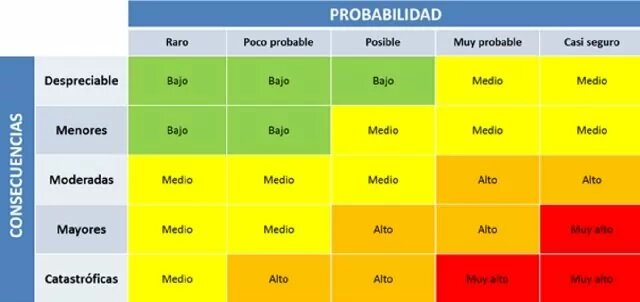
\includegraphics[height=5cm, width=16cm]{matriz_riesgos.jpg}
\end{center}


Los riesgos identificados para el desarrollo de este proyecto son:

\begin{itemize}
    \item Diseño de interfaz (No está definida con el cliente, probabilidad: casi seguro, consecuencias: mayores, riesgo: muy alto)
    \begin{itemize}
        \item Plan de contigencia: definir la interfaz con el cliente.
        \item Plan de atenuación: Estudiar con el cliente qué cambios se pueden realizar en la interfaz existente.
    \end{itemize}
    
    \item Falta de diseñadores (No está contemplado en el personal una persona especializada en UX, probabilidad: casi seguro, consecuencias: mayores, riesgo: muy alto)
    \begin{itemize}
        \item Plan de contigencia: Formar a un miembro del equipo de desarrollo como diseñador UX.
        \item Plan de atenuación: Contratar a un miembro del equipo de desarrollo como diseñador UX. 
    \end{itemize}

    \item Implementación nuevas funcionalidades (probabilidad: probable, consecuencias: moderado, riesgo: medio)
    \begin{itemize}
        \item Plan de contigencia: Subcontratar una empresa para realizar las nuevas funcionalidades.
        \item Plan de atenuación: Reunirse con el cliente para redefinir los plazos de entrega.
    \end{itemize}

    \item Calidad empresa subcontratada (probabilidad: poco probable, consecuencias: menores, riesgo: bajo)
    \begin{itemize}
        \item Plan de contigencia: Buscar la mejor compañía que se ajuste al presupuesto de las funcionalidades que puedan surgir.
        \item Plan de atenuación: Enviar un miembro del equipo a supervisar que dichas funcionalidades se estén implementando correctamente.
    \end{itemize}

    \item Baja productividad: (probabilidad: muy problable, consecuencias: moderadas, riesgo: alto)
    \begin{itemize}
        \item Plan de contigencia: Lograr que el ambiente de trabajo sea agradable.
        \item Plan de atenuación: Hablar con el personal afectado para acordar una solución.
    \end{itemize}

    \item Requisitos demasiado complejos (probabilidad: rara, consecuencias: mayores, riesgo: medio)
    \begin{itemize}
        \item Plan de contigencia: Revisar la especificación de funcionalidades acordadas con cliente. Formación del equipo de desarrollo.
        \item Plan de atenuación: Renegociar los plazos de entrega con el cliente.
    \end{itemize}

    \item Conocimientos del equipo (probabilidad: muy probable, consecuencias: catastróficas, riesgo: alto)
    \begin{itemize}
        \item Plan de contigencia: Formación del equipo impactado. Revisiones más periódicas.
        \item Plan de atenuación: Reemplazar al miembro del equipo afectado.
    \end{itemize}

\end{itemize}
\end{document}